\title{
	Chess \\
	\large User Manual}
\date{\vspace{-5ex}}
\documentclass{article}
\usepackage[utf8]{inputenc}
\usepackage{graphicx}
\graphicspath{ {images/} }

\begin{document}
\maketitle

\section*{Introduction}
So, you want to play chess? Well, you’ve come to the right place. Lets just get this straight: If you are not over the age of five, this game is not intended for you, unless you are mature for your age, then go ahead. 
If you are looking for a beginner stage in your chess career, this is a wonderful place for you to start. In this game you will be able to learn about the rules and different moves. If you think you are a skilled player you will be able to challenge yourself against the AI to become better. No matter how much you’ve played chess before, you will be able to become better and learn more about the game. Or if you’ve got a friend who needs to get of their high horse because they think they’re so much better than you, you can invite them to your house and play against them on your own computer. Or, if you're the lazy kind, just invite them to an online game.

\section*{Key Features}
If you choose to play against the computer you will be able to choose different difficulties: Easy, medium, hard. If you are a beginner, the easy difficulty is meant to help you learn basic chess, and help you get better by showing you possible moves with different pieces. If you think you’ve made the wrong move, you can regret your moves. There will also be an overview of all the moves made so far in the game. And don’t be afraid of making an illegal move, if you do a move that’s not legal, we won’t let you, and the piece will be put back to the previous position.  
If you choose medium or hard difficulty you will still have the option to use the hint button. The computer will try to beat you, and you will just have to counter it and try to beat it. 
You will always be able to see what your score is, and the pieces that you take of your opponent will be shown at the side. 
You also have the option of starting with a random board state. The pieces will be placed at random positions, with random number of pieces. So you can challenge yourself even more if you think you're too good for normal chess.
If you want to learn some different ways to put your opponent in checkmate, then fear not, there is hope for you. We've made a tutor that gives you certain board scenarios where you should be able to put your opponent in checkmate in three moves. There is only one ideal move for each round, and if you don't get the correct move, the board will reset and you will have to try again. 


\newpage
\section*{Rules}
What follows is the rules of each chess piece, and special moves allowed:

\subsection*{Check}
Check is a condition where the opponent can knock out your king within their next turn. Your opponent will say check.

\subsection*{Checkmate} Checkmate is a condition where the opponent can knock out your king and you have no options to move your king out of threat. Your opponent will say checkmate and you have lost the game.

\subsection*{Pawn} The pawn is the smallest soldier in the chess game. The pawn is not allowed to move far, and is only allowed to move forward. The first time you move a pawn you are allowed to move it two squares forward. When a pawn has been moved once, he’s only allowed to move one square forward each turn. In terms of knocking out the opponents chess pieces, the pawn is the only piece that doesn’t knock out in the direction it’s moving. If the pawn wants to knock out another piece it can only do so on square diagonally forwards to the right or to the left.
If you by some miracle manage to get the pawn all the way over to the opponents first row, you get a reward. The reward is that you can transform the pawn into any other chess piece.  
\begin{figure}[h]
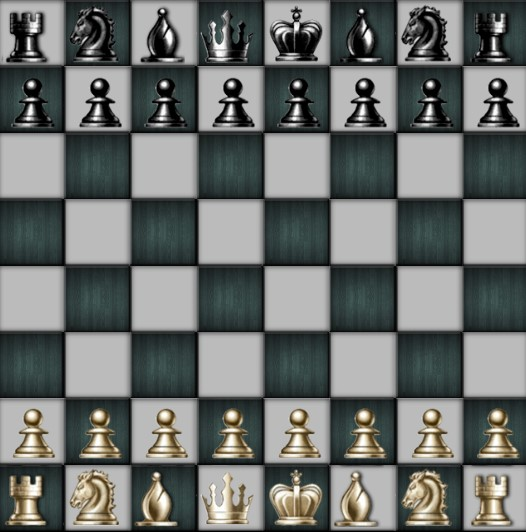
\includegraphics[width=3.5cm, height=4cm]{pawn1} 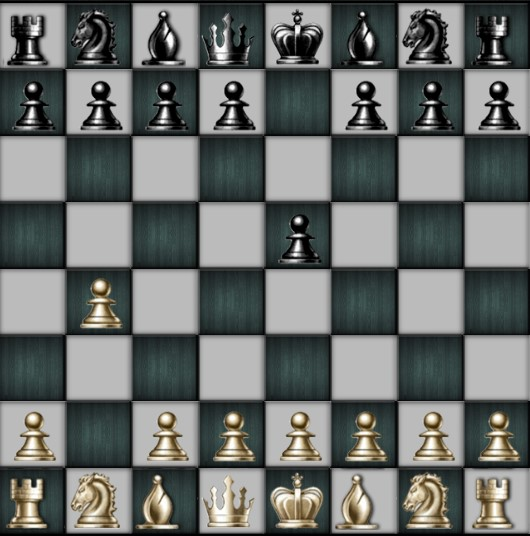
\includegraphics[width=3.5cm, height=4cm]{pawn2} 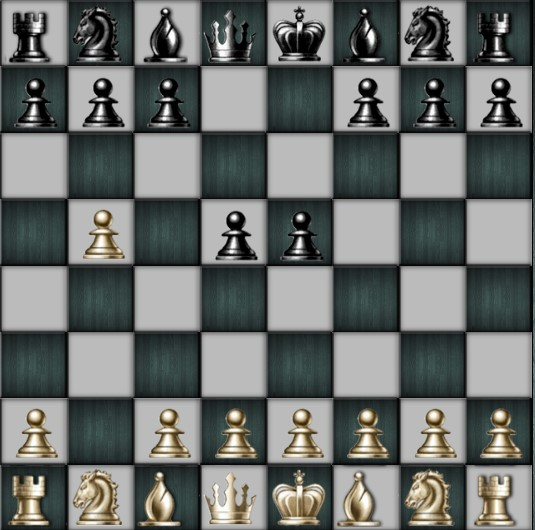
\includegraphics[width=3.5cm, height=4cm]{pawn3}
\end{figure}

\subsection*{Rook} If you need more firepower than the pawn, the rook is something else. As long as there’s no other piece in the way it’s moving, it can move as far as it pleases. The rook can only move in a straight line forwards, backwards and sideways, but not diagonally. The rook can’t change direction while moving, you have to choose a direction to move it in before moving. If there’s a piece from the opponent in the rooks way, the rook can knock the piece out, but it can’t move further than the piece it knocks out.
\begin{figure}[h]
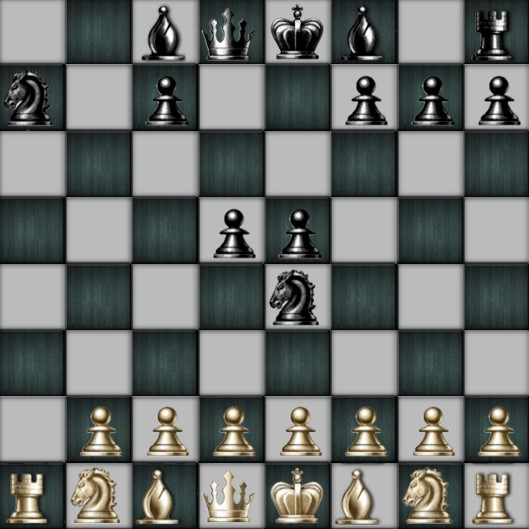
\includegraphics[width=5cm, height=5cm]{rook1}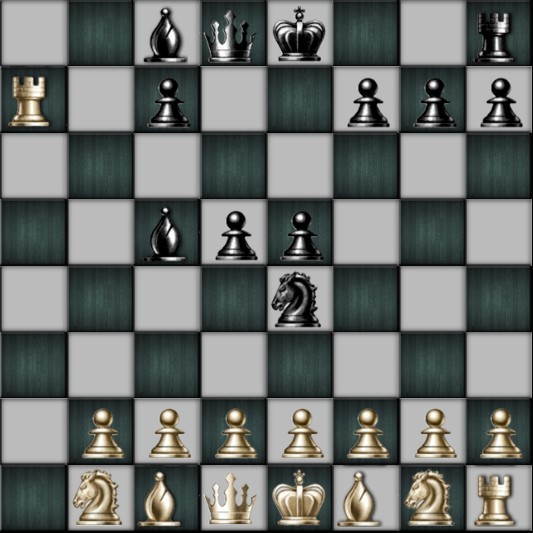
\includegraphics[width=5cm, height=5cm]{rook2} 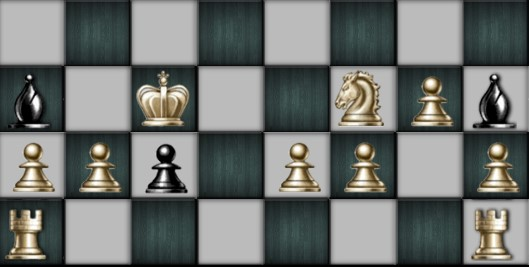
\includegraphics[width=5cm, height=5cm]{rook3} 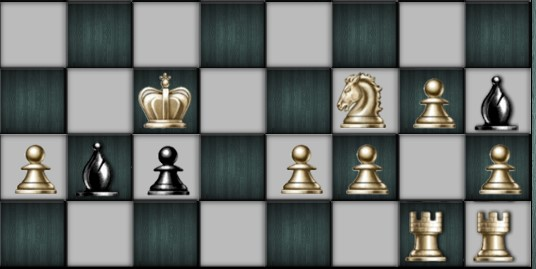
\includegraphics[width=5cm, height=5cm]{rook4}
\end{figure}

\subsection*{Bishop} The bishop is more limited in its movement than the rook, but it’s more useful than the pawn. The bishop can only move diagonally forwards or backwards. The bishop has the same principles as the rook in terms of how far it can move, and that it can’t change direction while moving. 
\begin{figure}[h]
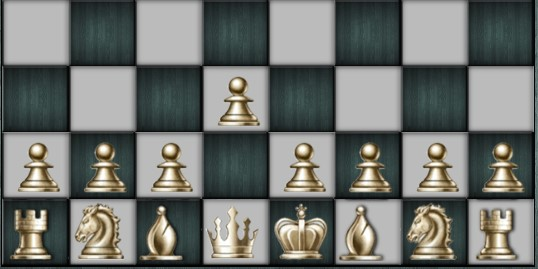
\includegraphics[width=6cm, height=3cm]{bishop1} 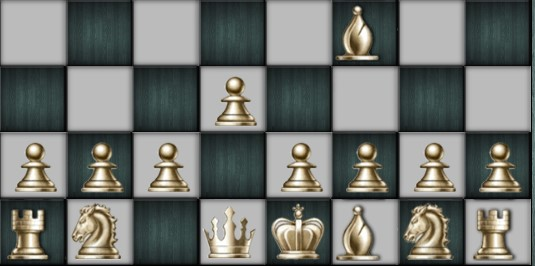
\includegraphics[width=6cm, height=3cm]{bishop2} 
\end{figure}

\subsection*{Knight} In terms of complexity, the knight is the worst. It doesn’t move in a straight line or in just one direction. The knight moves in a L-shape on the board. The knight always go two squares in one direction, and one square another direction, but that can still be confusing. There’s normally two different ways for the knight to get to a square, so sometimes you can move one square in one direction followed by two squares in another direction. Another unique quality about the knight is that it can jump over other pieces. Because of the knight’s special way of moving it doesn’t matter if there’s pieces in the way. If the knight wants to knock out a piece from the opponent, it has to land on the piece it wants to knock out.
\begin{figure}[h]
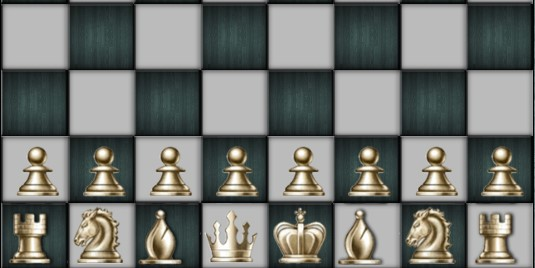
\includegraphics[width=3.9cm, height=4cm]{knight1} 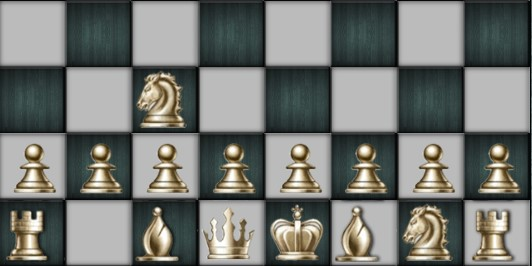
\includegraphics[width=3.9cm, height=4cm]{knight2} 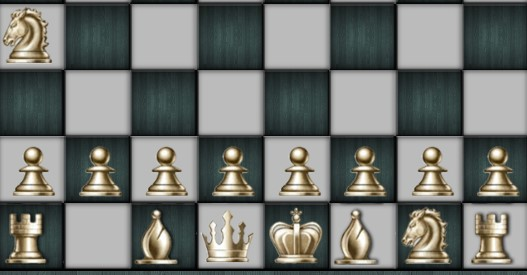
\includegraphics[width=3.9cm, height=4cm]{knight3}
\end{figure}

\subsection*{Queen} In terms of power, the queen is the most powerful chess piece on the board. If you combine the movement of the rook and the bishop, you get the movement of the queen. The queen can move as far as she wants, as long as there’s no other piece in the way, forwards, backwards, sideways and diagonally.
\begin{figure}[!]
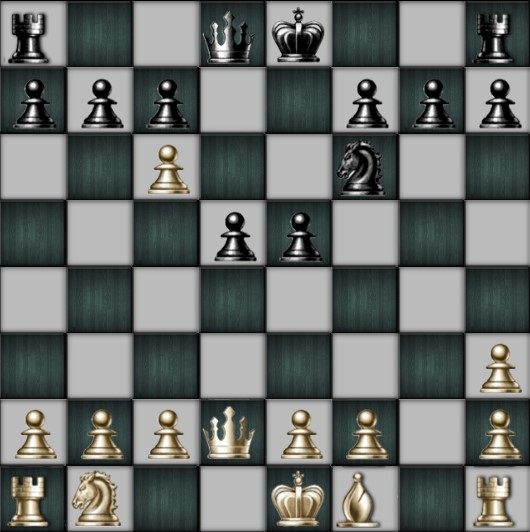
\includegraphics[width=5cm, height=5cm]{queen1}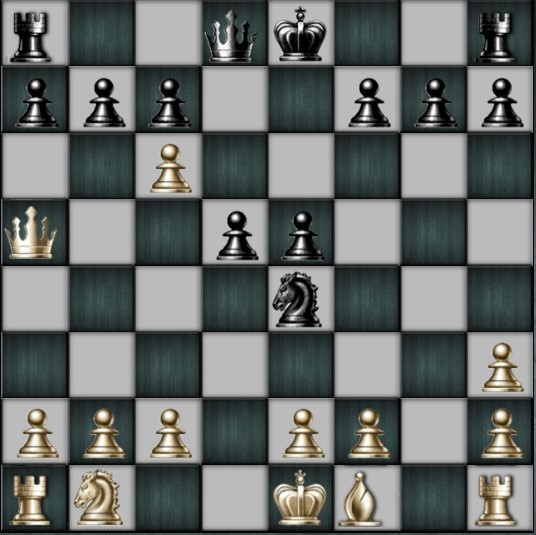
\includegraphics[width=5cm, height=5cm]{queen2}
\end{figure}

\begin{figure}[!]
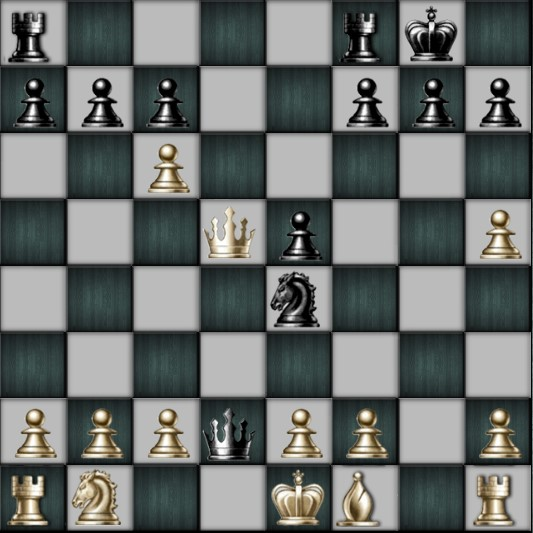
\includegraphics[width=5cm, height=5cm]{queen3}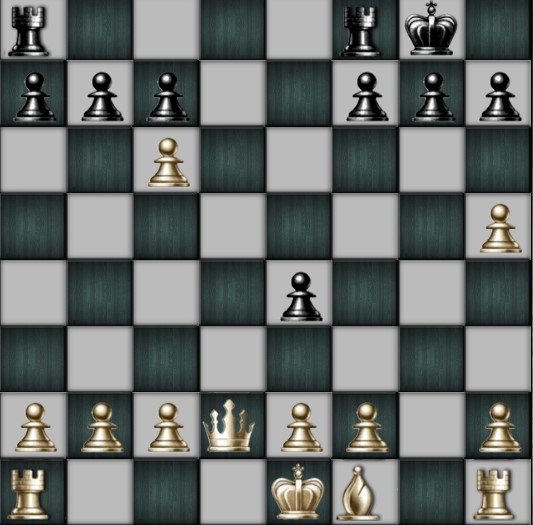
\includegraphics[width=5cm, height=5cm]{queen4}
\end{figure}
\subsection*{King} The most important piece on the board, is the king. That’s the piece you have to protect using the other pieces. If the king gets knocked out by your opponent, you loose. The kings movement is restricted to one square in each direction. You are not allowed to put the king in danger by moving it into check. If your opponent puts you into check, you are obliged to get the king out of danger. The opposing kings are not allowed to stand right next to each other, there has to be at least one square between them. 
\begin{figure}[h]
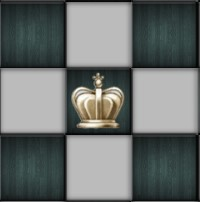
\includegraphics[width=4cm, height=4cm]{king1}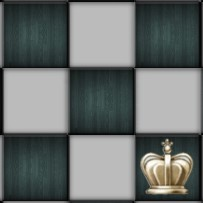
\includegraphics[width=4cm, height=4cm]{king2} 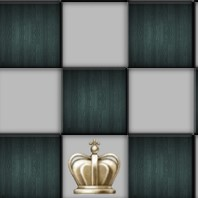
\includegraphics[width=4cm, height=4cm]{king3} 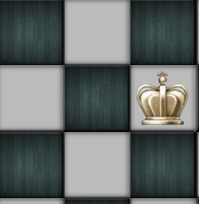
\includegraphics[width=4cm, height=4cm]{king4}
\end{figure}

\subsection*{Castling} To ensure safety of the king there are measures one can take. The most effective measure one can do is called castling. Castling involves two pieces, the king and the rook. In rough terms the king and the rook switches positions. The terms of castling are:
\begin{itemize}
	\item There has to be a clear path between the king and the rook; there can be no pieces in between them. 
	\item The king and the rook can not have been moved earlier in the game, they still have to be positioned in their starting position. 
	\item If the castling results in the king ending up being in check, castling is not allowed.
	\item If the king is checked, castling is not allowed.
	\item If one of the squares the king has to move through is controlled by an opponent piece, castling is not allowed. This is because it’s not allowed to expose the king to danger.
\end{itemize}
When castling occurs, the king moves two squares towards the rook it wants to do the castling with. When the king has moved two squares, the rook then jumps over the king and lands on the square next to the king, opposite of the side where it started.
There are two kinds of castling, short castling and long castling. Short castling is when the castling happens on the kings side of the board, long castling is when the castling happens on the queens side of the board.
\begin{figure}[h]
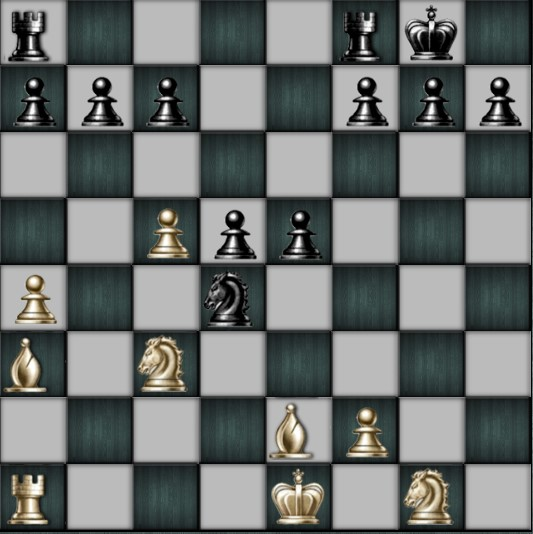
\includegraphics[width=6cm, height=6cm]{castling1} 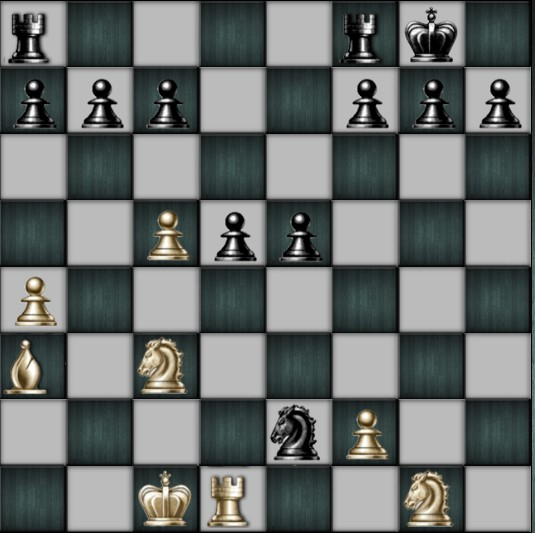
\includegraphics[width=6cm, height=6cm]{castling2} 
\end{figure}

\subsection*{En passant} A pawn has a secret ability in a special case. If a pawn gets to the fifth row, it gets an extra ability as an award for getting halfway over the board. This ability gives the pawn an opportunity to knock out an opponent pawn. The terms for en passant:
\begin{itemize}
	\item The pawn has to be on your fifth row. 
	\item The opponents pawn has to be on the column directly next to your own pawn and has to be on its starting position, and it has to move two squares forward so it’s positioned directly next to your pawn. 
	\item If you wish to knock out this pawn, you just have to pretend the pawn only had moved one square forward from its starting position, instead of two. So you move the pawn diagonally, but you don’t land on the same square as the pawn you knock out. 
	\item This has to be done immediately after the opponent moved its pawn two squares forward, otherwise you lose the opportunity to use en passant.
\end{itemize}
\begin{figure}[h]
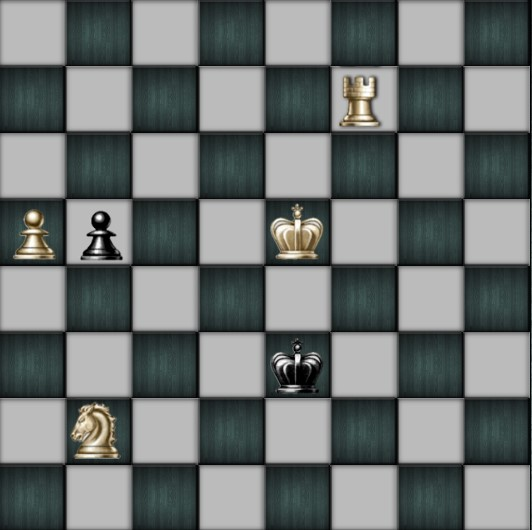
\includegraphics[width=6cm, height=6cm]{enpa1} 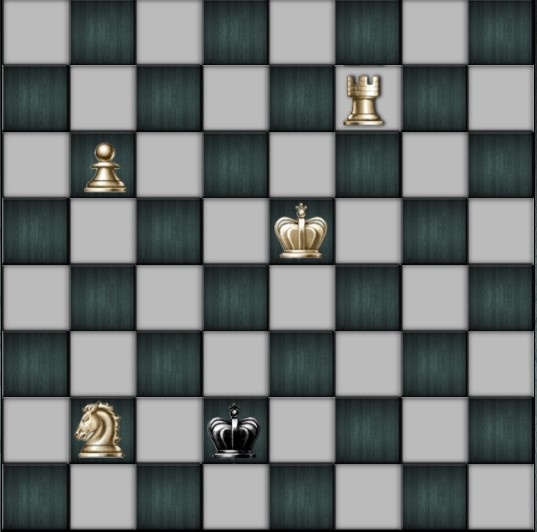
\includegraphics[width=6cm, height=6cm]{enpa2} 
\end{figure}

\end{document}